\documentclass[tikz,border=3pt]{standalone}
\usepackage{mathptmx}
\usetikzlibrary{arrows.meta,positioning,fit,backgrounds,calc,shapes.misc,decorations.pathreplacing}

\definecolor{acc}{RGB}{38,76,132}   % muted blue: harness / instrument structure
\definecolor{sig}{RGB}{178,52,42}   % muted red: regression / fail
\definecolor{ink}{RGB}{20,20,20}
\definecolor{mute}{RGB}{110,110,110}

\begin{document}
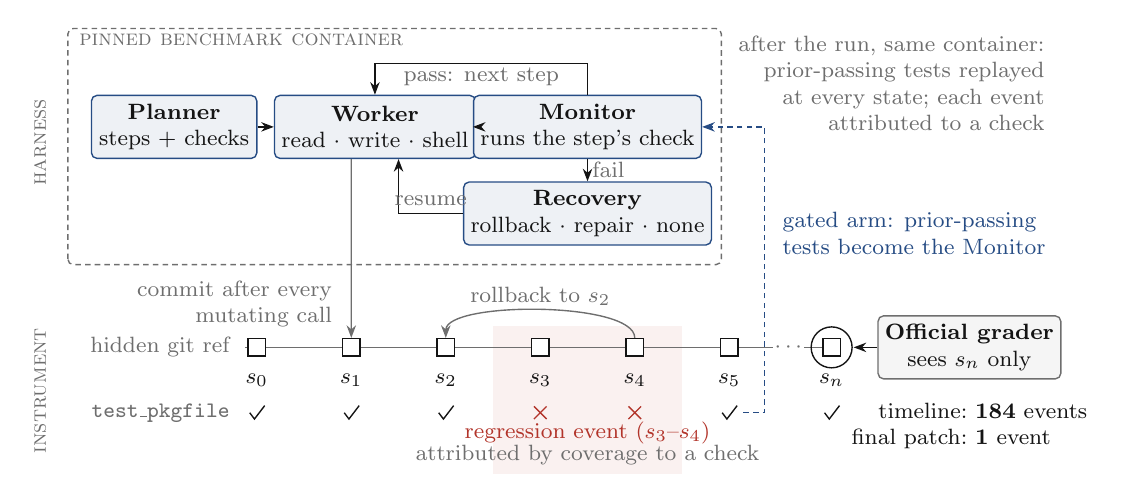
\begin{tikzpicture}[
  font=\footnotesize,
  line width=0.5pt,
  >={Stealth[length=1.6mm,width=1.2mm]},
  every node/.style={inner sep=2.5pt, text=ink},
  box/.style={draw=acc, fill=acc!8, rounded corners=2pt, line width=0.5pt,
              minimum width=2.1cm, minimum height=0.8cm, align=center},
  gbox/.style={draw=mute, fill=black!4, rounded corners=2pt, line width=0.5pt,
              minimum width=2.1cm, minimum height=0.8cm, align=center},
  flow/.style={draw=ink, ->},
  soft/.style={draw=mute, ->},
  gate/.style={draw=acc, ->, dashed, dash pattern=on 2pt off 1.5pt},
  lab/.style={text=mute},
  lane/.style={text=mute, rotate=90, anchor=center, font=\footnotesize\scshape},
  st/.style={draw=ink, fill=white, minimum width=2.2mm, minimum height=2.2mm, inner sep=0pt},
]

% ---------------- harness (top lane) ----------------
\node[lane] at (0.45,4.55) {harness};

\node[box] (planner) at (2.15,4.75) {\textbf{Planner}\\steps + checks};
\node[box] (worker)  at (4.70,4.75) {\textbf{Worker}\\read $\cdot$ write $\cdot$ shell};
\node[box] (monitor) at (7.40,4.75) {\textbf{Monitor}\\runs the step's check};
\node[box] (recov)   at (7.40,3.65) {\textbf{Recovery}\\rollback $\cdot$ repair $\cdot$ none};

\draw[flow] (planner) -- (worker);
\draw[flow] (worker) -- (monitor);
\draw[flow] (monitor.north) -- ++(0,0.4) -| (worker.north);
\node[lab, below, inner sep=1.5pt] at ($(worker.north)!0.5!(monitor.north)+(0,0.4)$) {pass: next step};
\draw[flow] (monitor.south) -- node[right, lab, inner sep=1.5pt] {fail} (recov.north);
\draw[flow] (recov.west) -| node[above, lab, pos=0.25] {resume} ([xshift=3mm]worker.south);

% container boundary
\draw[draw=mute, dashed, dash pattern=on 2pt off 1.5pt, rounded corners=2pt]
  (0.8,3.0) rectangle (9.1,6.0);
\node[lab, anchor=west, font=\footnotesize\scshape] at (0.85,5.85) {pinned benchmark container};

% ---------------- instrument (bottom lane) ----------------
\node[lane] at (0.45,1.4) {instrument};

% commit drop
\draw[soft] ([xshift=-3mm]worker.south) -- (4.4,2.07);
\node[lab, align=right, anchor=east] at (4.25,2.5) {commit after every\\mutating call};

% regression window shading
\fill[sig!7] (6.2,0.34) rectangle (8.6,2.22);

% baseline with axis break before s_n
\draw[draw=mute] (3.05,1.95) -- (9.75,1.95);
\draw[draw=mute] (10.15,1.95) -- (10.5,1.95);
\node[lab, inner sep=0pt] at (9.95,1.95) {$\cdots$};

% states
\foreach \x/\l in {3.2/0, 4.4/1, 5.6/2, 6.8/3, 8.0/4, 9.2/5, 10.5/n} {
  \node[st] at (\x,1.95) {};
  \node[inner sep=0pt, anchor=north] at (\x,1.62) {$s_{\l}$};
}
% row labels
\node[lab, anchor=east] at (2.95,1.95) {hidden git ref};
\node[lab, anchor=east] at (2.95,1.12) {\texttt{test\_pkgfile}};

% replay glyphs: pass at s0-s2, fail at s3-s4, pass at s5 and s_n
\foreach \x in {3.2, 4.4, 5.6, 9.2, 10.5} {
  \draw[draw=ink] (\x-0.09,1.12) -- (\x-0.03,1.04) -- (\x+0.1,1.21);
}
\foreach \x in {6.8, 8.0} {
  \draw[draw=sig] (\x-0.08,1.04) -- (\x+0.08,1.20);
  \draw[draw=sig] (\x-0.08,1.20) -- (\x+0.08,1.04);
}
\node[text=sig] at (7.4,0.86) {regression event ($s_3$--$s_4$)};
\node[lab] at (7.4,0.58) {attributed by coverage to a check};

% rollback arc
\draw[soft] (8.0,2.07) to[out=90,in=90,looseness=0.5] node[above, lab, pos=0.5, inner sep=1.5pt] {rollback to $s_2$} (5.6,2.07);

% gated arm feedback: the prior-passing tests become the Monitor
\draw[gate] (9.38,1.12) -- (9.65,1.12) |- (monitor.east);
\node[text=acc, anchor=west, align=left] at (9.78,3.4) {gated arm: prior-passing\\tests become the Monitor};

% grader
\draw[draw=ink] (10.5,1.95) circle (0.26);
\node[gbox] (grader) at (12.25,1.95) {\textbf{Official grader}\\sees $s_n$ only};
\draw[flow] (grader.west) -- (10.78,1.95);
\node at (12.25,0.95) {\begin{tabular}{@{}r@{\ }l@{}}
  timeline: & \textbf{184} events \\
  final patch: & \textbf{1} event
\end{tabular}};

% operational note (what the instrument does, after the run)
\node[lab, anchor=north east, align=right] at (13.3,6.0)
  {after the run, same container:\\prior-passing tests replayed\\at every state; each event\\attributed to a check};

\end{tikzpicture}
\end{document}
